%adobe reader fix
\pdfminorversion=4

\documentclass[final]{beamer}

%set image/logo options
% Rice
\def\RightLogoWidth{0.18}
\def\RightLogoPaddingTop{0.25cm}
\def\RightLogoPaddingBottom{0.5cm}
\def\RightLogo{../logos/RiceLogo_TMCMYK300DPI.jpg}
% SHINE
\def\LeftLogoWidth{0.17}
\def\LeftLogoPaddingTop{0.5cm}
\def\LeftLogoPaddingBottom{0.5cm}
\def\LeftLogo{../logos/shine-logo.png}
% SunPy
\def\AnotherLeftLogoWidth{0.06}
\def\AnotherLeftLogoPaddingTop{0.25cm}
\def\AnotherLeftLogoPaddingBottom{0.25cm}
\def\AnotherLeftLogo{../logos/sunpy_powered_logo.png}
% Title and author(s) block
\def\TitleWidth{0.55}
% GitHub
\def\GitHubLogoWidth{0.014\paperwidth}
\def\GitHubLogo{../logos/GitHub-Mark-120px-plus.png}
\def\GitHubUser{wtbarnes}
% Affiliation in footer
\def\AffiliationFooter{Department of Physics and Astronomy - Rice University - Houston, TX USA}
% Email
\def\EmailAddressFooter{will.t.barnes@rice.edu}

%set theme
\mode<presentation>
{
\usetheme{I6dv_custom}
}
\setbeamertemplate{caption}[numbered]

%Include packages
\usepackage{soul,color,verbatim}
\usepackage{type1cm}
\usepackage{calc}
%\usepackage{times,mathptmx}
\usepackage{amsmath,amsthm,amssymb,latexsym}
\usepackage{empheq}
\usepackage{graphicx}
\usepackage{epstopdf}
\usepackage[numbers]{natbib}
\usepackage{multicol}
\usepackage{subfigure}
\usepackage[english]{babel}
%\usepackage[latin1]{inputenc}
\usepackage{tikz}
%setup beamerposter package
\usepackage[orientation=portrait,size=custom,width=91.44,height=121.92,scale=1.0]{beamer/beamerposter/beamerposter}

%tikz configuration

%custom commands go here
\newcommand{\ang}{\AA~} %alias angstrom
\setbeamerfont{caption}{size=\footnotesize} %make caption size small

%Set author and title
\title[Observable Signatures of Nanoflares]{Modeling Observable Signatures of Nanoflare Heating\\Frequency in Active Region Cores}
\author[Barnes \& Bradshaw]{Will T. Barnes \& Stephen J. Bradshaw}
\institute[Rice University]{Department of Physics and Astronomy\\Rice University}
\date{24-28 July, 2017}

%start poster
%everything goes in one frame
\begin{document}
\begin{frame}
  %start columns environment to slice up the page horizontally
  \begin{columns}[T]
  \hfill
  %%
  %%first column
  \begin{column}{0.49\linewidth}
    %introduction
    \begin{block}{Introduction}
    \vspace{-1ex}
    \begin{itemize}
      \item Nanoflare model of \citet{parker_nanoflares_1988}: corona heated by impulsive ($\ll\tau_{cool}$), low-energy ($10^{24}$ erg) events produced by twisting, braiding of field lines rooted in the photosphere
      \item Fundamental question: \alert{what is the frequency of energy release in the solar corona?}
      \item Define heating frequency in terms of $t_N$,      
      \begin{itemize}
        \item Low-frequency heating: Time between successive events is much greater than typical loop cooling time (i.e. approaches single nanoflare case), $t_N>\tau_{cool}$ low-frequency heating
        \item High-frequency heating: Time between successive events is much smaller than typical loop cooling time (i.e. approaches steady heating case), $t_N<\tau_{cool}$ high-frequency heating
      \end{itemize}
      \item \textbf{Goal:} \alert{Use hydrodynamic loop models to better understand how different heating properties}
      \item What is the frequency of nanoflares in AR cores?
      \item Emission measure slope $\mathrm{EM}\sim T^a,\,\,6.0<\log{T}<\log{T_{peak}}$ often used as a diagnostic for heating frequency
      \item Many factors hinder interpretation
      \begin{itemize}
        \item Multiple emitting structures along the LOS
        \item Nonequilibrium ionization
        \item Inversion techniques for finding EM
        \item Lack of spectral coverage in detectors
      \end{itemize}
      \item Two primary questions:
      \begin{itemize}
        \item What are the observational signatures of nanoflares of varying frequency?
        \item Are these signatures detectable?
      \end{itemize}
    \end{itemize}
    \end{block}
    % forward modeling
    %% Describe synthesizAR code, maybe a diagram?
    \begin{block}{Forward Modeling}
      \vspace{-1ex}
      \begin{itemize}
      \item Foo
      \item Bar
      \end{itemize}
    \end{block}
    % Heating model
    %% Show tN distributions
    \begin{block}{Heating Model}
      \begin{columns}[T]
      \begin{column}{0.49\columnwidth}
        \begin{itemize}
        \item Each strand heated independently
        \item Preferentially heat electrons
        \item Triangual pulses with duration $\tau=200$ s
        \item Total input energy per strand set by 
              \begin{equation*}
                E = \frac{(\epsilon B)^2}{8\pi}
              \end{equation*}
        \item $B$ is the average field strength per strand determined by the field extrapolation
        \item Event energies chosen from a power-law distribution with $\alpha=-2.5$
        \item $t_{N,i}\propto E_i$ such that larger events require a longer ``winding time''
        \end{itemize}
      \end{column}
      \begin{column}{0.49\columnwidth}
        \begin{figure}
        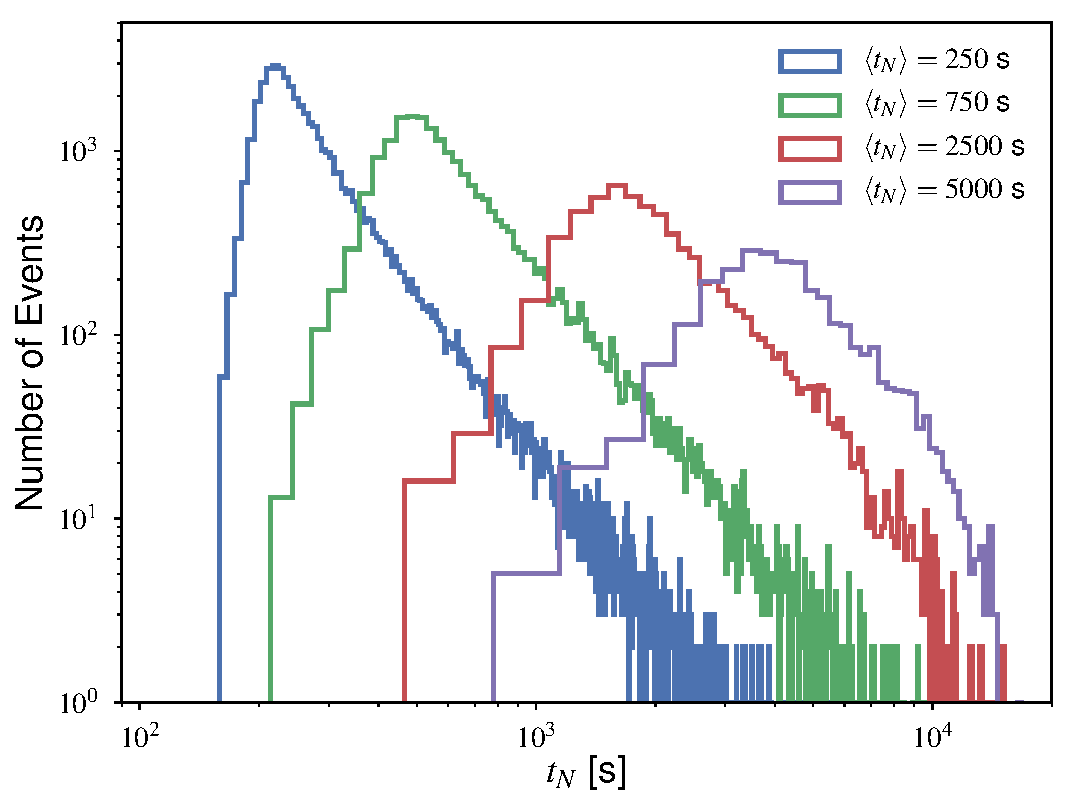
\includegraphics[width=\columnwidth]{figures/wait_time_distributions.pdf}
        \caption{Distribution of wait times for four different heating frequencies}
        \label{fig:wait_times}
        \end{figure}
      \end{column}
      \end{columns}
    \end{block}
    % Spectroscopic details/atomic physics
    %% What lines are we modeling? 
    \begin{block}{Spectroscopic Details}
      \begin{columns}[T]
        \begin{column}{0.49\columnwidth}
          \begin{figure}
            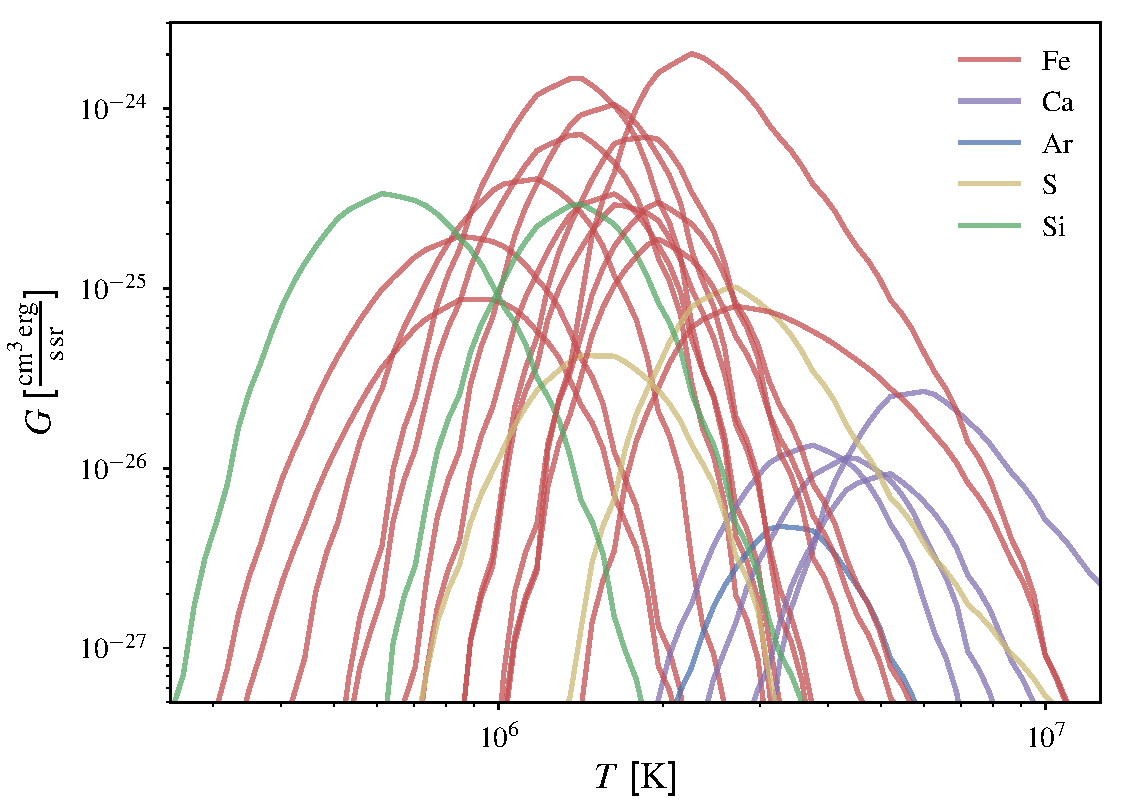
\includegraphics[width=\columnwidth]{figures/contribution_functions.pdf}    
          \end{figure}
        \end{column}
        \begin{column}{0.49\columnwidth}
        \begin{table}
\begin{tabular}{cc}
Ion & Wavelength \\
 & $\mathrm{\mathring{A}}$ \\
Fe XV & 284.163 \\
Fe XIV & 264.789 \\
Si VII & 275.361 \\
Ca XVI & 208.585 \\
Fe XIV & 270.521 \\
Fe XIII & 202.044 \\
Fe XIII & 203.826 \\
S X & 264.231 \\
Fe XVI & 262.976 \\
Fe IX & 188.493 \\
Fe IX & 197.854 \\
Ar XIV & 194.401 \\
Fe XII & 195.119 \\
Fe XII & 192.394 \\
Ca XIV & 193.866 \\
Fe XI & 188.216 \\
S XIII & 256.685 \\
Fe X & 184.537 \\
Si X & 258.374 \\
Fe XI & 180.401 \\
Ca XV & 200.972 \\
Ca XVII & 192.853 \\
\end{tabular}
\end{table}

        \end{column}
      \end{columns}
    \end{block}
    % EM diagnostics
    %% how to calculate true versus predicted EM
    \begin{block}{Emission Measure Diagnostics}
      \begin{itemize}
        \item \textit{True} emission measure from simulated thermodynamic quantities,
              \begin{equation*}
                \mathrm{EM}(T) = \int_{\mathrm{LOS}}\mathrm{d}h\,n^2(h,T)
              \end{equation*} 
        \item Bin in temperature $5.6<\log{T}<7.0$ with width $\Delta\log{T}=0.05$
        \item \textit{Predicted} EM from regularized inversion code of \citet{hannah_differential_2012}
        \begin{itemize}
          \item Assume 25\% uncertainty on our intensities to balance acceptable $\chi^2$ and smoothness
        \end{itemize}
        \item Fit power-law to cool side such that $\mathrm{EM}\sim T^a$
        \begin{itemize}
          \item Fit between 1 MK and $T_{peak}$ (4 MK true, 3 MK predicted), where $\mathrm{EM}_{max}=\mathrm{EM}(T_{peak})$
          \item Only fit to pixels where $\mathrm{EM}(T)>10^{25}\,\,\mathrm{cm}^{-5}$ and acceptable fit $R^2>0.95$
        \end{itemize}
      \end{itemize}
    \end{block}
  \end{column}
  %%
%%%%%%%%%%%%%%%%%%%%%%%%%%%%%%%%%%%%%%%%%%%%%%%%%
  %%second column
  \begin{column}{0.49\linewidth}
    % em distributions
    %% maps of true versus predicted EM for a all tN and a few T bins
    \begin{block}{Emission Measure Distributions}
      \begin{itemize}
      \item Foo
      \item Bar
      \end{itemize}
    \end{block}
    % em slopes
    %% maps of em slopes
    \begin{block}{Emission Measure Slopes}
      \begin{itemize}
      \item Foo
      \item Bar
      \end{itemize}
      \vspace{-1ex}
    \end{block}
    % em slope distributions
    %% distribution of slopes plus overplotted results from literature
    \begin{block}{Slope Distributions}
    \end{block}
    %Conclusions
    \begin{block}{Conclusions}
      \begin{itemize}
      \item Some
      \item conclusions
      \item here
      \end{itemize}
    \end{block}
    %references
    \begin{block}{References}
      \scriptsize
      \vspace{-2ex}
      \begin{multicols}{2}
        \bibliographystyle{apj}
        \bibliography{references.bib}
      \end{multicols}
    \end{block}
  \end{column}
  \end{columns}
\end{frame}
\end{document}
